\chapter{Reference abstract hardware architecture}

\section{Why a reference abstract hardware architecture?}

For proper understanding of openETCS API and of constraints imposed on
both sides of the API, we need to define a \emph{reference abstract
  hardware architecture}. This hardware architecture is ``abstract''
is the sense that the actual vendor specific hardware architecture
might be totally different of the abstract architecture described in
this chapter. For example, several units might be grouped together on
the same processor.

However the actual vendor specific architecture shall fulfill all the
requirements and constraints of this reference abstract hardware
architecture and shall not request additional constraints.

\section{Definition of the reference abstract hardware architecture}

\begin{figure}
  \centering
  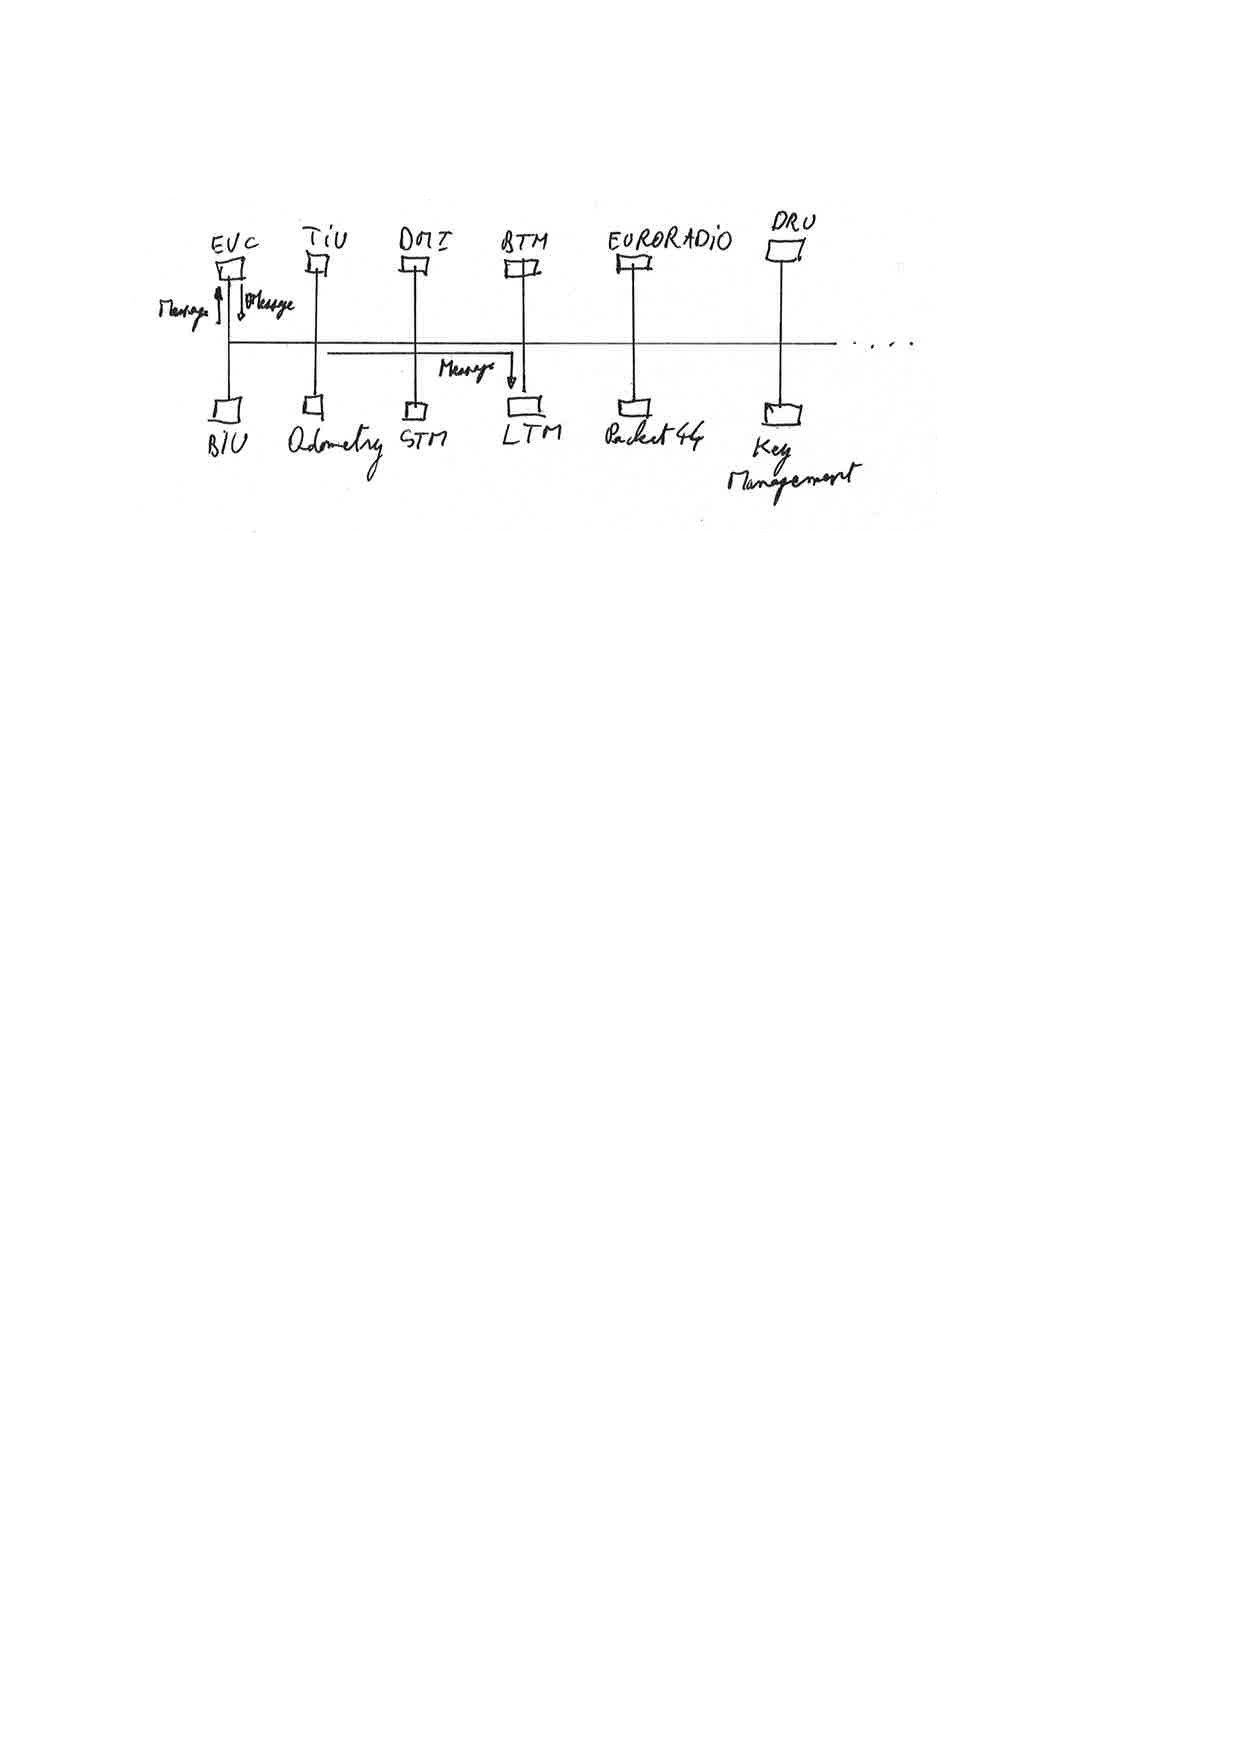
\includegraphics{abstract-hardware-architecture.pdf}
  \caption{Reference abstract hardware architecture}
  \label{fig:hardware-arch}
\end{figure}

The reference abstract hardware architecture is shown in figure
\ref{fig:hardware-arch}.

The reference abstract hardware architecture is made of a bus on which
are connected physical units:
\begin{itemize}
\item EVC (European Vital Computer);
\item BIU;
\item TIU (Train Interface Unit);
\item Odometry;
\item DMI (Driver Machine Interface);
\item STM (Specific Transmission Module);
\item BTM (Balise Transmission Module);
\item LTM (Loop Transmission Module);
\item EURORADIO;
\item Packet 44 (Alstom Transport specific module, \cite{alstom-api});
\item DRU (Diagnostic Recording Unit, Alstom Transport specific
  module, \cite{alstom-api});
\item Key Management (Alstom Transport specific module,
  \cite{alstom-api});
\item Other units.
\end{itemize}

A given instance of openETCS might not have all of above
units. \FIXME{Define a set of mandatory units?}

Those units shall working concurrently. They shall exchange
information with other units through asynchronous message passing.

% LocalWords:  Alstom openETCS EVC BIU TIU Odometry DMI STM BTM Balise LTM API
% LocalWords:  EURORADIO
